%%%%%%%%%%%%%%%%%%%%%%%%%%  ltexpprt.tex  %%%%%%%%%%%%%%%%%%%%%%%%%%%%%%%%
%
% This is ltexpprt.tex, an example file for use with the SIAM LaTeX2E
% Preprint Series macros. It is designed to provide double-column output.
% Please take the time to read the following comments, as they document
% how to use these macros. This file can be composed and printed out for
% use as sample output.

% Any comments or questions regarding these macros should be directed to:
%
%                 Donna Witzleben
%                 SIAM
%                 3600 University City Science Center
%                 Philadelphia, PA 19104-2688
%                 USA
%                 Telephone: (215) 382-9800
%                 Fax: (215) 386-7999
%                 e-mail: witzleben@siam.org


% This file is to be used as an example for style only. It should not be read
% for content.

%%%%%%%%%%%%%%% PLEASE NOTE THE FOLLOWING STYLE RESTRICTIONS %%%%%%%%%%%%%%%

%%  1. There are no new tags.  Existing LaTeX tags have been formatted to match
%%     the Preprint series style.
%%
%%  2. Do not change the margins or page size!  Do not change from the default 
%%     text font!
%%
%%  3. You must use \cite in the text to mark your reference citations and
%%     \bibitem in the listing of references at the end of your chapter. See
%%     the examples in the following file. If you are using BibTeX, please
%%     supply the bst file with the manuscript file.
%%
%%  4. This macro is set up for two levels of headings (\section and
%%     \subsection). The macro will automatically number the headings for you.
%%
%%  5. No running heads are to be used for this volume.
%%
%%  6. Theorems, Lemmas, Definitions, etc. are to be double numbered,
%%     indicating the section and the occurence of that element
%%     within that section. (For example, the first theorem in the second
%%     section would be numbered 2.1. The macro will
%%     automatically do the numbering for you.
%%
%%  7. Figures, equations, and tables must be single-numbered.
%%     Use existing LaTeX tags for these elements.
%%     Numbering will be done automatically.
%%
%%  8. Page numbering is no longer included in this macro.
%%     Pagination will be set by the program committee.
%%
%%
%%%%%%%%%%%%%%%%%%%%%%%%%%%%%%%%%%%%%%%%%%%%%%%%%%%%%%%%%%%%%%%%%%%%%%%%%%%%%%%



\documentclass[twoside,leqno,twocolumn]{article}
\usepackage{ltexpprt}

\usepackage{times}
\usepackage{ulem}
\usepackage{amsmath}
\usepackage{algorithm}
\usepackage[noend]{algpseudocode}
%\usepackage[vlined,ruled]{algorithm2e}
\usepackage{tikz}
\usepackage{graphicx}
\usepackage{float}
\usepackage[inline]{enumitem}
\usetikzlibrary{positioning,shapes,arrows,fit,automata}
\usepackage{natbib}
\begin{document}

\makeatletter
\def\BState{\State\hskip-\ALG@thistlm}
\makeatother

%\setcounter{chapter}{2} % If you are doing your chapter as chapter one,
%\setcounter{section}{3} % comment these two lines out.
\newcommand*\samethanks[1][\value{footnote}]{\footnotemark[#1]}
\title{\Large Robust resource demand estimation using hierarchical Bayesian model in a distributed service system}
\author{ {Sumanta Mukherjee\thanks{IBM Research - India}} \\
\and
{ Krishnasuri Narayanam\samethanks}  \\
\and
{Digbalay Bose\thanks{University of Southern California, CA, U.S.}}   \\
\and 
{Nupur Aggarwal\samethanks[1]} \\
\and
{Amith Singhee\samethanks[1]}
}

\date{}

\maketitle

% Copyright Statement
% When submitting your final paper to a SIAM proceedings, it is requested that you include 
% the appropriate copyright in the footer of the paper.  The copyright added should be 
% consistent with the copyright selected on the copyright form submitted with the paper.
% Please note that "20XX" should be changed to the year of the meeting.

% Default Copyright Statement
\fancyfoot[R]{\scriptsize{Copyright \textcopyright\ 2018 by SIAM\\
Unauthorized reproduction of this article is prohibited}}

% Depending on which copyright you agree to when you sign the copyright form, the copyright 
% can be changed to one of the following after commenting out the default copyright statement
% above.

%\fancyfoot[R]{\scriptsize{Copyright \textcopyright\ 20XX\\
%Copyright for this paper is retained by authors}}

%\fancyfoot[R]{\scriptsize{Copyright \textcopyright\ 20XX\\
%Copyright retained by principal author's organization}}


%\pagenumbering{arabic}
%\setcounter{page}{1}%Leave this line commented out.

\begin{abstract} \small\baselineskip=9pt 
Robust resource demand prediction is crucial for efficient allocation of resources to service requests in a distributed service delivery system. There are two problems in resource demand prediction: firstly to estimate the volume of service requests that come in at different time points and at different geolocations, secondly to estimate the resource demand given the estimated volume of service requests. While a lot of literature exists to address the first problem, in this work, we have proposed a data-driven statistical method for robust resource demand prediction to address the second problem. The method automates the identification of various system operational characteristics and contributing factors that influence the system behavior to generate an adaptive low variance resource demand prediction model. Factors can be either continuous or categorical in nature. The method assumes that each service request resolution involves multiple tasks. Each task is composed of multiple activities. Each task belongs to a task type, based on the type of the resource it requires to resolve that task. Our method supports configurable tasks per service request, and configurable activities per task. The demand prediction model produces an aggregated resource demand required to resolve all the activities under a task by activity sequence modeling; and aggregated resource demand by resource type, required to resolve all the activities under a service request by task sequence modeling.
\end{abstract}


\section{Introduction}
\label{sec:intro}
In a distributed service delivery system, a response to a service request often involves multiple tasks. These tasks are often dependent on each other in sequential order. Dependence order among the tasks is restricted by the service delivery industry domain.  Different service requests can be of different types. The type of a service request is defined by a combination of tasks. Further, a task is defined by a combination of activities. Each task is carried out by one or more resources of a specific resource type. All the activities associated with a task are carried out by the same resource type.
\par
A proactive response in such a service delivery system requires estimation of upcoming resource demand at activity resolution across all service requests. Demand estimation is done over a specified time interval. The specific composition of task types defining a service request type is explicitly modeled in our method. And the specific composition of activities defining a task type is also explicitly modeled in our method. Activity is the finest level of granularity of specifying the resource demand. For example, in an electrical utility, the service request is equivalent to a reported power outage. Resources represent the skilled human resources involved in resolving the service requests. Based on the work type, there can be multiple resource types, viz. repair crew, and assessment crew. A service request may involve multiple tasks based on the type of the service request. Each task involves multiple activities, viz., acquire tools, travel to the location, and work at the site.
\par
There are two distinct aspects to this problem, firstly estimating the number of incoming service requests, and secondly, for a given volume of requests estimating the resource demand. The first aspect of the problem can be solved using time-series analysis. But it's not possible to solve the second part using time-series analysis, as the time series models are incapable of producing a sequence of activities with dependency constraints, which is essential for the resource demand estimation. This estimation process involves a high degree of uncertainty, inherent to the system. 
\par
Here we will discuss a novel Hierarchical Bayesian Network model for robust estimation of the resource demand profile for a given set of service requests.


\section{Related work}
\label{sec:literature}
Resource demand estimate for service request resolution under emergency is needed for any service delivery organization for faster resolution of the service requests. \cite{H.Li} addressed the problem of risk management of electrical outages by using a Poisson regression model for spatial data in a hierarchical Bayesian framework. During a severe weather event, a Tobit model-based system was proposed by \cite{Amith} for estimating number of outages in a distribution grid. \cite{Zhiguo} tackled the problem of forecasting weather-driven damages of different types by combining a spatial clustering based scheme with data from multiple weather networks. A combination of weather-based simulations, land-cover and outage utility data was used by \cite{Wanik} to calibrate various ensemble-based methods for predicting the spatial distribution of outages in Northeastern USA. Another application of ensemble-based methods was explored by \cite{Padm}, where a boosting-based technique called Adaboost$+$ was designed for estimating wind and lightning related outages.
\par
In \cite{Mallik}, a statistical model based on weather forecasts, asset information, historical damage patterns and geography was built for predicting localized interruptions  and was subsequently used by National Grid in its emergency planning efforts. \cite{Trenish} also combined calibrated weather models with historical damage data to design a forecast model for outages. An integrated system called OPRO (Outage Prediction and Response Optimization) \cite{OPRO} was proposed for emergency situations in terms of weather events by integrating weather and damage predictions with resource planning and health aware damage hot-spot analysis. \cite{Lubkeman} developed a decision support tool based on the model of distribution circuit layout, the placement of protective and switching devices and the location of customers for resource allocation and management. \cite{Lee2009} in their work have proposed a simulation based modeling framework to analyze the optimal point of distribution under emergency situation. 
\par
A predictive method that utilizes different weather data in a GIS framework was developed for outage maintenance by \cite{Chen}. The GIS framework in-spite of providing the advantage of handling geo-spatial data efficiently, fails during the time of extreme weather events due to non-availability of location information. \cite{Wu} explored a fuzzy logic based methodology for crew management in case of large scale multiple outages. A similar approach was considered by \cite{PCChen} where both weather related forecasts and power-system based operational data were integrated with a fuzzy logic approach to aid the outage maintenance system. An unsupervised approach based on ensemble learning method was designed by \cite{Salehi} for predicting the damage of extreme events like wildfires in Australia. 
\par
In spite of this large gamut of literature none precisely addressed the problem of robust demand estimation along with a structure of task/activity order dependency. The method can address modeling of any system that conforms to the desired process ontology (as in section~\ref{sec:definition}).  

\section{Definitions}
\label{sec:definition}
In order to produce a generalized model across various systems, we have designed a descriptive process template. Each service request is broken down into a sequence of tasks. Each task resolution involves a sequence of activities. Demand is attributed to each activity. Demand is described in terms of resource hours. E.g., If the activity demand is 8 units, it means that a resource need to spend 8 hours to complete that activity. Equivalently, it takes 4 hours for 2 resources working on the same activity together. The system takes the expected number of service requests ($R$) over a period of time as input, and produces spatio-temporal resource demand profile over that period ($D$). The service requests are distributed over geolocation, and arrive at different times. The split of the service requests ($R$) into their corresponding tasks is represented as ($T$), and the split of the all the tasks ($T$) into their corresponding activities is presented as ($A$). 
\par
For each activity, there is a distinct resource demand associated. Demand associated with an activity is affected by few observed variables or attributes, which we call as factors ($\mathbf{F}$) in our modeling. The factors can be external ($E$) and internal ($I$). Generally, external factors ($E$) remain constant during the period of service request resolution. Internal factors ($I$) represent variables that are associated with the service request, task, or activity (Figure~\ref{fig:ontology}). 
\par
In an electric utility distribution grid, terrain specifics of the outage location, time of the year, time of the day, weather condition are examples of external factors. Equipment associated with an outage, severity of an outage, type of task are examples of internal factors. Internal factors are only known post the service request resolution.
\par
The model assumes a causality relationship between these entities, viz. factors, service requests, tasks, activities, and demands. Imposing this causality restriction helps to disambiguate the dependency order between these entities. Figure~\ref{fig:ontology} depicts this dependency. Assume that $I_R$, $I_T$, and $I_A$ are the internal factors associated with the service requests ($R$), tasks ($T$), and activities ($A$) respectively. $E$, and $R$ are observed entities (i.e., input) at the time of demand estimation (highlighted with double circled nodes in Figure~\ref{fig:ontology}). $T$, and $A$ are generated using sequence models. $R$, $T$, and $A$ represent the volume estimate of work at different granularity and are shown as nodes in black in Figure~\ref{fig:ontology}.  Modeling of $T$ is dependent on $E$ and $I_R$. Modeling of $A$ is dependent on $E$ and $I_T$. The demand estimate ($D$) is obtained using hierarchical Bayes model (marked blue in Figure~\ref{fig:ontology}), which intern uses all factors ($E$, $I$). Modeling of internal factors ($I_R$, $I_T$, and, $I_A$) is always dependent on external factors ($E$) (all the factor nodes are marked in red in Figure~\ref{fig:ontology}). Details of the internal factor modeling, and demand estimation are explained in the section~\ref{sec:method}. 

\begin{figure}[t]
	\centering
	\resizebox{0.8\columnwidth}{!}{
	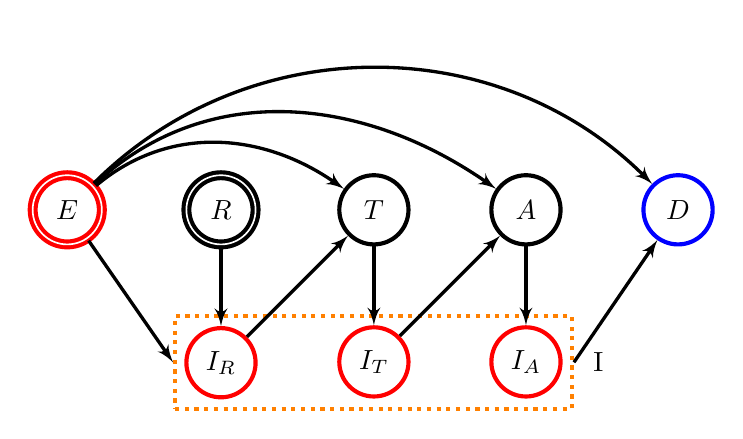
\begin{tikzpicture}
	\begin{scope}[line width=1.5]
	\node[state, accepting, draw=red] (E) {$E$};
	\node[state, accepting, right=of E, draw=black] (R) {$R$};
	\node[state,right=of R, draw=black] (T) {$T$};
	\node[state,right=of T, draw=black] (A) {$A$};
	\node[state,right=of A, draw=blue] (D) {$D$};
	\node[state,below=of R, draw=red] (IR) {$I_R$};
	\node[state,below=of T, draw=red] (IT) {$I_T$};
	\node[state,below=of A, draw=red] (IA) {$I_A$};
	\end{scope}
	\node[draw=orange,dotted,fit=(IR) (IT) (IA),line width=1.5] (I) {};
	\node[right=of I, xshift=-25] (Itag) {I};
	\begin{scope}[line width=1.2]
	\draw[-latex'] (R) -- (IR);
	\draw[-latex'] (T) -- (IT);
	\draw[-latex'] (A) -- (IA);
    \draw[-latex'] (E) -- (I.west);
	\draw[-latex'] (IR) -- (T);
    \draw[-latex'] (E) to[out=40,in=145] (T);
	\draw[-latex'] (IT) -- (A);
	\draw[-latex'] (E) to[out=43,in=145] (A);
	\draw[-latex'] (I.east) -- (D);
	\draw[-latex'] (E) to[out=45,in=135] (D);
	\end{scope}
	\end{tikzpicture}
	}
	\caption{Process template, and causal dependencies.}
    \label{fig:ontology}
\end{figure}

\section{Methods}
\label{sec:method}
Demand prediction for a set of input service requests ($R$) happens via two phases: training, and scoring. In the training phase, statistical model parameters are estimated using the historical data. Here historical data includes details about the service requests, their corresponding tasks, activities, and resource demand along with the associated external factors. In the scoring phase, using the derived statistical model, demand is estimated for each activity that corresponds to the set of input service requests.
\par 
The non-parametric statistical analysis of the resource demand often exhibits multi-modal behavior. If the modes are distinct and well separated, we call them operating characteristics. There may be one or more operating characteristics associated with a input set of service requests. 
\par The training phase includes 4 major sub-phases: 
\begin{enumerate*}
	\item Identification of contributing factors to distinct operating characteristics, and partitioning the training data for regression model building,
	\item Conditional sequence generator modeling, 
    \item Generative models for internal factor estimation, and
	\item Identification of crucial factors and robust regression model estimation for resource demand.
\end{enumerate*}
\par
Scoring step uses the trained model obtained in the training phase, along with the expected volume of the service requests and the observed values of external factors to produce the expected resource demand profile ($D$). Scoring step performs a series of prediction tasks in the order of entity dependencies in the process template (Figure~\ref{fig:fig2a}). Three types of computation are involved in the scoring phase:
\begin{enumerate*}
\item Expected task sequence estimation, and activity sequence estimation, 
\item Estimation of internal factors, and
\item Demand estimation using regression model
\end{enumerate*}.

%The prediction results are produced in a tabular format as two tables:
%\begin{enumerate*}
%\item Predecessor and successor tasks generated using sequence modeling (task generation). This table describes all pairs of tasks, which have a temporal dependency (e.g., a successor task can not be started without completing it's predecessor task), and
%\item Resource demand estimate for each task at activity level
%\end{enumerate*}.

\begin{figure*}[t]
 \centering
 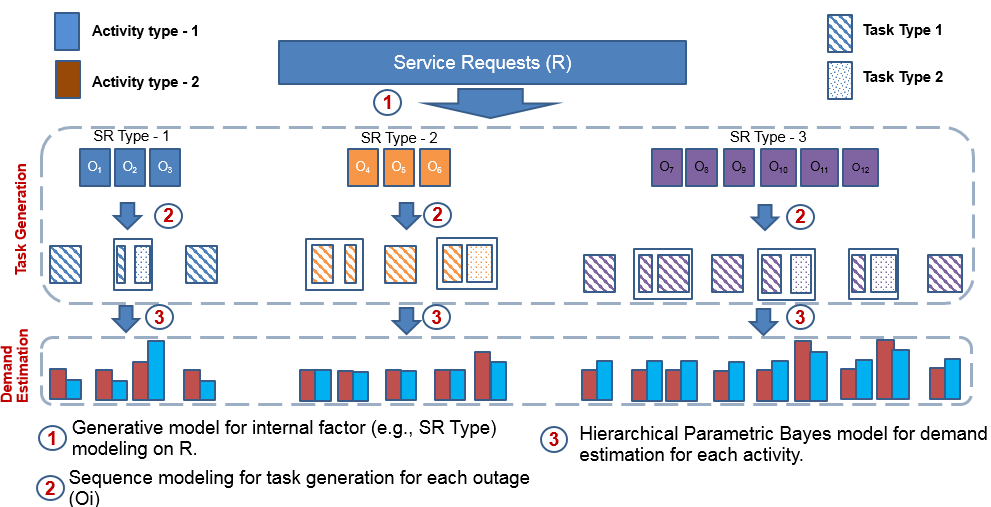
\includegraphics[width=16cm]{fig2a}
 \caption{Steps in the activity based demand estimation method. $O_i$ is used to represent an outage (i.e., a service request). Service request type (i.e., SR Type) is the factor considered here.}
 \label{fig2a}
\end{figure*}

\subsection{Input}\label{subsec:input}
Inputs to the training are:
\begin{enumerate*}
	\item historical data,
	\item input specification.
\end{enumerate*}
 Historical data is a set of $N$ records. Each record composed of values for different data items, e.g., service request, task, activity, task type, task dependency, associated process attributes etc. The input specification explicitly describes the correspondence between each entry of record to the process template. The historical data is transformed to map to a set of tuples ${\lbrace t_{R}^{i}, t_{T}^i, t_{A}^{i}, E_{1}^{i},\dots E_{k}^{i}, P_{1}^{i},\dots,P_{m}^{i}, R^{i}, T^{i}, A^{i}, D^{i} \rbrace }_{i=1 \dots N}$, where $t_{R}^{i}$,$t_{T}^{i}$, and $t_{A}^{i}$ represent the respective starting time-stamps for service request, tasks, and activities of each historical data entry. $E^{i}$ represents various external factors, $P^{i}$, $R^{i}$, $T^{i}$, $A^{i}$, and $D^{i}$, are associated parameters, service request, tasks, activities and resource demand respectively. In a electric utility distribution grid, examples of a parameter are service request type, service request arrival time, task type, equipment used, cause of the outage, etc. These parameters are used to derive the internal factors ($I$) in our method.

\subsection{Identification of distinct operating characteristics}
\label{subsec:characteristic}
In order to produce a low variance demand estimation model, the demand profile of the training data is analyzed for identification of multi-modality or distinct operating characteristics. The multi-modality is associated with operating characteristics only when it is possible to identify an unique factor, that best explains the multi-modal behavior (Figure~\ref{fig2}). Our model imposes a strong association for any operating characteristic with only one factor, in order to identify the appropriate statistical model during demand estimation step. To evaluate the contribution of a factor to the distinct operating characteristics, the data is partitioned into non-intersecting chunks by factor value. If $F_i$ represents a factor which can take possible values $\lbrace f_{i,1}, f_{i,2} \dots f_{i,k} \rbrace$, then the data $\mathbf{X}$ is partitioned into $k$ non-intersecting sets $X_1 , \dots X_k$, where $X_{j} = \lbrace x: F_i(X) = f_{i,j} \rbrace $ and $j \in \{1,2,...,k\}$.
\par 
Kolmogorov-Smirnov (KS)'s two sample test identifies the max separation between two non-parametric cumulative distributions
\begin{equation*} 
 \gamma_{m,n} = \max_{x}{\vert G_{m}(x) - G_{n}(x) \vert}
\end{equation*}
where, $G_{m}$ and $G_{n}$ are two cumulative distributions derived from input data partitions $m$ and $n$ respectively. KS distance ($\gamma_{m,n}$) is symmetric and satisfies metric properties~\cite{degroot2002}. 

\begin{figure}[t]
	\centering
	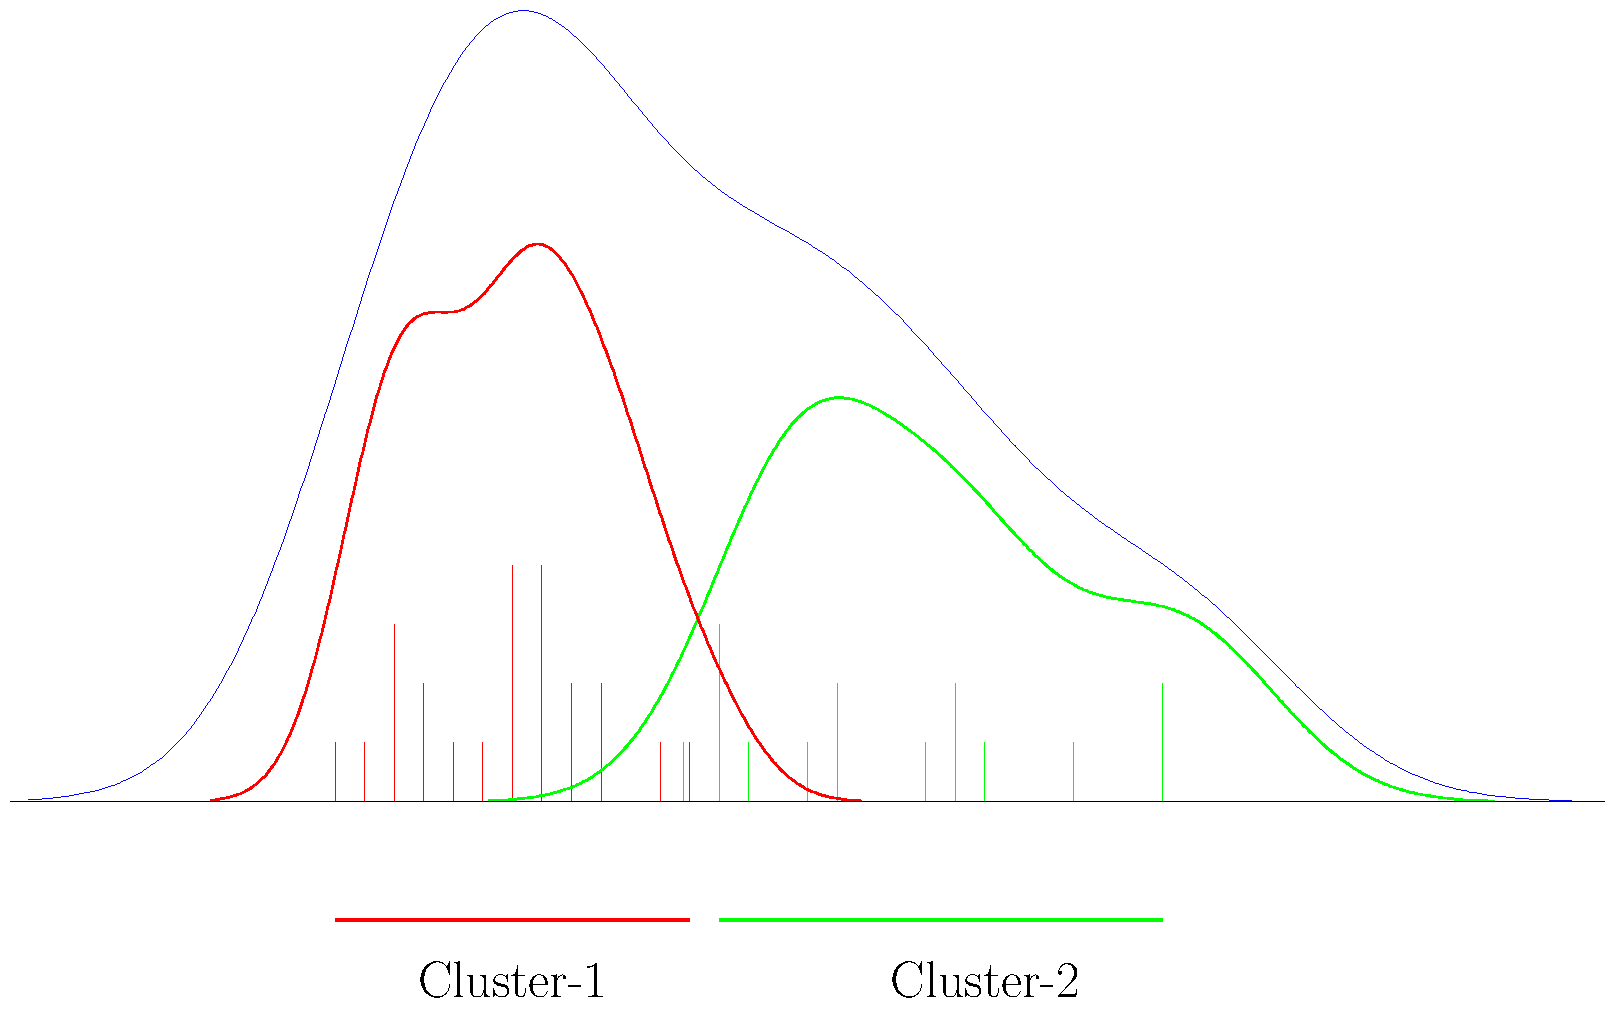
\includegraphics[width=8cm]{fig2.pdf}
	\caption{Sample partitioning of data points into two clusters. Factor values are similar, in each cluster.}
    \label{fig2}
\end{figure}

 KS distance is evaluated between all partition pairs. $\delta_{D}$ is a decision parameter used to decide whether the KS distance obtained is significant for operating characteristic identification. In order to ascertain the significance of the KS distance we impose a minimum sample size ($\mathbf{N}$) requirement on each partition. Using the distance measure $\Gamma(X\vert F_i) = \Big[\gamma_{X_i,X_j}\Big]_{i,j}$, a hierarchical cluster is obtained ($\mathbf{H}(F_i\vert\Gamma)$). At a distance cutoff of $\delta_{D}$, the cluster partitions are marked. This partitions the factor $F_i$ values into non-overlapping groups $\mathcal{C}^{1}_{F_i},\dots,\mathcal{C}^{u}_{F_i}$, such that KS distance between any two factor values in the same partition is $< \delta_{D}$, while between any two factor value across partitions is $\geq \delta_{D}$. 
\par
The sup norm of the evaluated distance matrix ( ${\vert\vert \Gamma(X\vert F_i) \vert\vert}_{\infty}$ ) is marked as factor association score to operating characteristics. The factor with maximum association score ($\geq \delta_{D}$), is considered as the explanatory factor.
\par
Explanatory factor identification, splits the training data into non-intersecting partitions. For each data partition, above method of finding operating characteristics is repeated, till no distinct operating characteristics are found. 

\subsection{Conditional sequence generator}
\label{subsec:seqgen}
Total resource demand forecast ($\mathbf{D}$) is an aggregated demand across all activities. 
\begin{eqnarray*}
\mathbf{D} & = & \sum_{r}{ \sum_{t\in \mathcal{T}(r,F)}{ \sum_{a\in\mathcal{A}(t,F)}{ D(a,t,r,F) } } } 
\end{eqnarray*} 
In above expression, $r$ iterates over list of all incoming service requests. $\mathcal{T}(r,F)$, and $\mathcal{A}(t,F)$ are task sequence generator and activity sequence generators respectively, and both these sequence generators are influenced by external and internal factors $F$ (i.e., $ E \cup I$).  
\par
We have used Markov chain approach for the activity sequence and task sequence modeling~\cite{kemeny2012}. A typical Markov chain is an infinite length sequence generator. In the current context, task and activity sequences are of finite length. To address the same, we introduce two pseudo states, viz., start state ($s$)  and end state ($e$) (Figure~\ref{markov}). Any sequence generated by this Markov chain model is of type ($s \dots e$). The Markov chains are represented with transition matrix $\mathcal{M}$, which is learned from the historical data using Markov training process. 
\begin{figure}
\centering
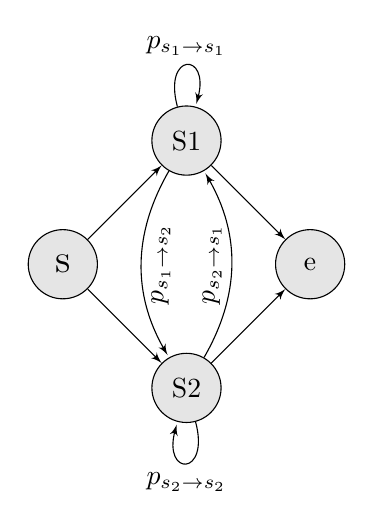
\begin{tikzpicture}
	\tikzset{node style/.style={state, minimum width=0.75cm, fill=gray!20!white}}
	\node[node style,draw=black] (s) at (0,0) {\Large s};
	\node[right=of s] (dummy) {};
	\node[node style,above=of dummy] (s1) {S1};
	\node[node style,below=of dummy] (s2) {S2};
	\node[node style, right=of dummy] (e) {e};
	\draw[-latex'] (s) -- (s1);
	\draw[-latex'] (s) -- (s2);
	\draw[-latex'] (s1) -- (e);
	\draw[-latex'] (s2) -- (e);
	\draw[every loop, auto=right, >=latex', draw=black]
	   (s1) edge[loop above] node {$p_{s_1 \rightarrow s_1}$} (s1)
	   (s2) edge[loop below] node {$p_{s_2 \rightarrow s_2}$} (s2)
	   (s1) edge[bend right,auto=left] node {\rotatebox{90}{$p_{s_1 \rightarrow s_2}$}} (s2)
	   (s2) edge[bend right,auto=left] node {\rotatebox{90}{$p_{s_2 \rightarrow s_1}$}} (s1);
\end{tikzpicture}
\caption{Finite state generator using Markov model.}
\label{markov}
\end{figure}
Causal dependence between the factors restricts the factor selection for task sequence generator and activity sequence generator modeling. Influential factor selection for sequence generator is a computationally expensive process. For every factor ($F_i$), first the data is partitioned by the factor value association. Markov transition matrix is estimated on each sub-partition. $\mathcal{M}(X\vert\mathbf{F}_{i,j})$, represents the Markov transition matrix derived for $j^{th}$ value of the factor $F_{i}$, from a given data $X$. The distance between given pair of Markov transition matrices ($\mathcal{M}_i$, and $\mathcal{M}_j$) is defined as `Frobenius` norm of difference matrix~\cite{Horn:2012}.
\begin{equation*}
d(\mathcal{M}_i,\mathcal{M}_j) = \sqrt{\text{trace}{\Big((\mathcal{M}_i - \mathcal{M}_j)}^{T}(\mathcal{M}_i - \mathcal{M}_j)\Big)}
\end{equation*}
The influence of a factor $F_i$ on the task sequence or activity sequence ($\mathcal{I}(X\vert\mathbf{F_i} )$) is estimated as the maximum distance from all pairs of transition matrices derived from the partitions for factor ($F_i$).
\begin{equation*}
\mathcal{I}(\mathbf{X\vert F_i}) = \max_{j \neq k} d\Big(\mathcal{M}(X\vert\mathbf{F}_{i,j}), \mathcal{M}(X\vert\mathbf{F}_{i,k})\Big)
\end{equation*}  
Factors are ranked using influence score. Top $\ell$ factors are used for final sequence generator modeling. $\ell$ is a model regularization parameter. Factors are categorical in nature, separate sequence generator models are derived for different combination of influencing factor values.

\subsection{Demand estimation model}
\label{subsec:demand}
Deriving the dependency graph is the crucial step in the demand estimation model. Dependency graph incorporates the causal dependency as described in the process template, and also captures statistical association between all entities. Dependency graph is computed multiple times during the training phase. It is used for internal factor modeling, and for resource demand modeling. For internal factor modeling, a single dependency graph is generated for all factors using the complete training data. In resource demand modeling, distinct dependency graphs are derived for each activity demand under each operating characteristic partition.

\subsubsection{Dependency Graph}
\label{subsubsec:graph}
Mutual information (MI) is used to identify statistical association between any pair of entities. The challenge here is the factors are categorical, while the demands are continuous. A nearest-neighbor based method is used for accurate estimation of MI~\cite{ross_mutual_2014}. A normalized mutual information (NMI) measure is used for system-wide analysis~\cite{EstevezTPZ09}. NMI between two random variables $X$ and $Y$ is defined as, 
\begin{equation*}
NMI(X;Y)=\dfrac{I(X;Y)}{ \text{min}( H(X) , H(Y) )}
\end{equation*}
where $I(X;Y)$ represents the mutual information between variables $X$, and $Y$; $H(X)$, and $H(Y)$ represent the information entropy for variables $X$ , and $Y$ respectively. The NMI is evaluated between every pair of entities $E$, $I$ and $D$. In a dependency graph, each vertex represents either a factor or a demand variable. An edge between node pairs describes the statistical association in terms of NMI as edge-weight. A direction is assigned to each edge by causal dependency compliant with process template.

\subsubsection{Internal factor modeling}
\label{subsubsec:factor}
Dependency graph with all factors is the backbone for internal factor modeling. Full training data is used to derive this dependency graph.  $\ell$ is a model regularization parameter; i.e., the maximum number of factors that can be used in modeling of an internal factor is $\ell$. Only top $\ell$ in-coming edges are used in factor modeling. For each internal factor modeling, a joint distribution is generated from the data $X$. Let's assume an internal factor $F_{i}$ can take $k$ distinct values, viz. $f_{i,1}, f_{i,2},\dots, f_{i,k}$. $F_{i1}, F_{i2},\dots F_{i\ell}$, are the modeling factors for $F_{i}$ derived from dependency graph. The generative statistical model for internal factor $F_{i}$ captures the conditional probability distribution $\mathrm{P}(F_i\vert F_{i1}, F_{i2},\dots F_{i\ell})$.

\subsubsection{Hierarchical Bayesian Estimation}
\label{subsubsec:hbm}
A Hierarchical Bayesian model (HBM) is used for resource demand modeling. A distinct HBM model is derived for each activity, and its operating characteristics. First using the variable dependency graph for a demand associated with an activity ($D_a$), statistical association of factors to $D_a$ are identified. Top $\ell$ influencing factors are used in the modeling. Factors are further ranked by their NMI value with $D_a$ in descending order. The training data is then recursively partitioned using the factor values in the rank order in a hierarchical fashion. The root node represents the set of all entries of $D_a$. In the next level, each partition represents a set of values of $D_a$  associated with a unique factor value. Similarly, the subsequent data partitions are obtained with respective factor values in a ranked order.  In the hierarchical data partition, the data size reduces exponentially with increasing depth of the partition tree.
\par  
In HBM, parameter estimation is carried out in top-down fashion. First the statistical distribution is obtained for the root partition. For root node, maximum likelihood estimate (\textit{MLE}) is used for the parameter estimation. In subsequent partition, parameter estimation is carried out using Bayesian model, with prior on the statistical parameters derived using the root partition statistics, $\mathbf{P}(\theta \vert X) \propto \mathbf{P}(X\vert\theta)\mathbf{P}(\theta)$~\cite{gelman2013}. This process ensures derivation of robust statistics less sensitive to outliers even with sparse data (Algorithm~\ref{algo2}).

\begin{algorithm}
\caption{Hierarchical Bayes Model}
\label{algo2}
\begin{algorithmic}[1]
\Procedure{Recursive Parameter Estimation}{}
\State Data set ${\lbrace x_i \rbrace}_{i=1\dots N}$
\State Parameter from parent distribution ${\theta}_{p}$
\State Sample bootstrap count $N_{b}$
\State $\Theta \leftarrow \emptyset$
\For {$i \in \lbrace 1 \dots N_b \rbrace $}
   \State $x_{s} \leftarrow \text{sample}( N \vert {\theta}_{p})$
   \State ${\theta}_{s} \leftarrow \textit{MLE}(x_s)$
   \State {$\Theta \leftarrow \lbrace \Theta, \theta_s \rbrace$ } 
\EndFor
\State $\alpha \leftarrow \textit{MLE}(\Theta)$
\State {${\theta}_{e} \leftarrow \textit{MAP}(\theta \vert x_i, \alpha)$} \Comment{$\theta$ is the search parameter}
\State \textbf{return} ${\theta}_{e}$
\EndProcedure
\end{algorithmic}
\end{algorithm}

\subsection{Model Execution}
Demand estimation, and task/activity sequence modeling are carried out in parallel. Both these analysis derive their own factor dependency graphs. Finally, factor dependency graphs, and influential factors for sequence models are merged together to yield the final factor dependency graph (Figure~\ref{fig3}). Factor dependency graph is the guideline for the order of execution of different models in the scoring phase. At the end of the training process, the final derived model includes following components 
\begin{enumerate*}
	\item factor dependency graph,
    \item generative model for internal factors,
	\item sequence generator models for task and activity,
	\item hierarchical Bayesian models for resource demand estimation.
\end{enumerate*}

\begin{figure}[t]
\centering
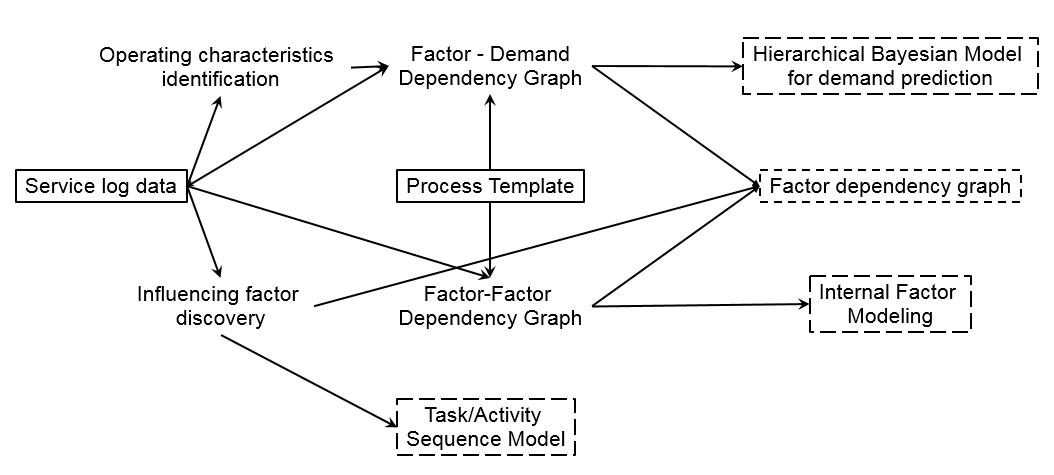
\includegraphics[width=8cm]{fig3}
\caption{Schematic of various concepts in our method, and their execution order dependency. Solid boxes are the inputs to the training phase. The dashed boxes are the final produced models.}
\label{fig3}
\end{figure}

In the scoring phase, for a new input with expected volume of service requests and their associated external factors, the model estimates internal factors in the order of their dependency, as described by the factor dependency graph.  Internal factor modeling often involves sequence modeling of tasks and activities. Once all the dependent factors are estimated, resource demand estimation is carried out using the hierarchical Bayesian model. 

\subsection{Sequence Generator}
\label{subsec:generator}
Let's assume, $\mathcal{M}$ represents the Markov transition matrix for sequence generation, and $\eta$ represents a feasible state in $\mathcal{M}$. Probability of $l$-th state being $\eta$, can be written in a dynamic programming formulation as,
\begin{eqnarray*}
\mathbf{p}(\eta,l) & = & \sum_{x}{\mathbf{p}(x,l-1)\mathcal{M}(x,\eta) } 
\end{eqnarray*}
Boundary condition to this formulation is at $l=0$, $\mathbf{p}(s,0) = 1$. $\mathcal{M}$ is a stochastic matrix; i.e., for any $l$, $\sum_{x}{\mathbf{p}(x,l)} = 1$. But the end state ($e$), is an absorbing state, i.e., $\mathbf{p}(e,e) = 1$. The probability of $\mathbf{p}(e,l)$ monotonically increases with increasing $l$. With the length of finite sequence generated using the Markov sequence model exhibits an exponential decay. Assume a simple single state system. The state space of the Markov transition matrix, contains three states $\lbrace s, \eta, e \rbrace$. Assume $p$ represents the transition probability from state $\eta \rightarrow \eta$. Then the probability vector of $l$-th state over three respective states can be analytically derived as $( 0, p^{l-1}, 1. - p^{l-1})\; \forall\; l > 1$.    

\section{Experimental Results}
In this section, we empirically demonstrate the predictive capability of our methods. Few experiments have been designed carefully to demonstrate the model accuracy. We have used field data collected from a representative electric utility distribution grid to analyze the prediction accuracy of the model. The field data is three year worth activity log of attended electrical outage service requests. The data has over 3,50,000 entries, where each entry corresponds to activities associated with a unique task. 

\subsection{Time series analysis of resource demands and service requests}\label{subsec:timeseries}
We analyzed the incoming volume of service requests, and resource demands on a daily basis using an auto-regressive integrated moving average (ARIMA) model on the historical data of major event days. In both the cases, we consider the last 6 months data as a hold-out set, and the remaining data for estimating the optimal model parameters. While forecasting over the duration of last 6 months, we employ a non-overlapping window of 3 days for augmenting the training data and provide the forecasts 3 days at a time. The quality of the forecasts for both resource demands and service requests is checked via RMSE values across multiple service delivery locations of the sample electrical utility described above.
\begin{figure*}
\centering
\begin{tabular}{cc}
 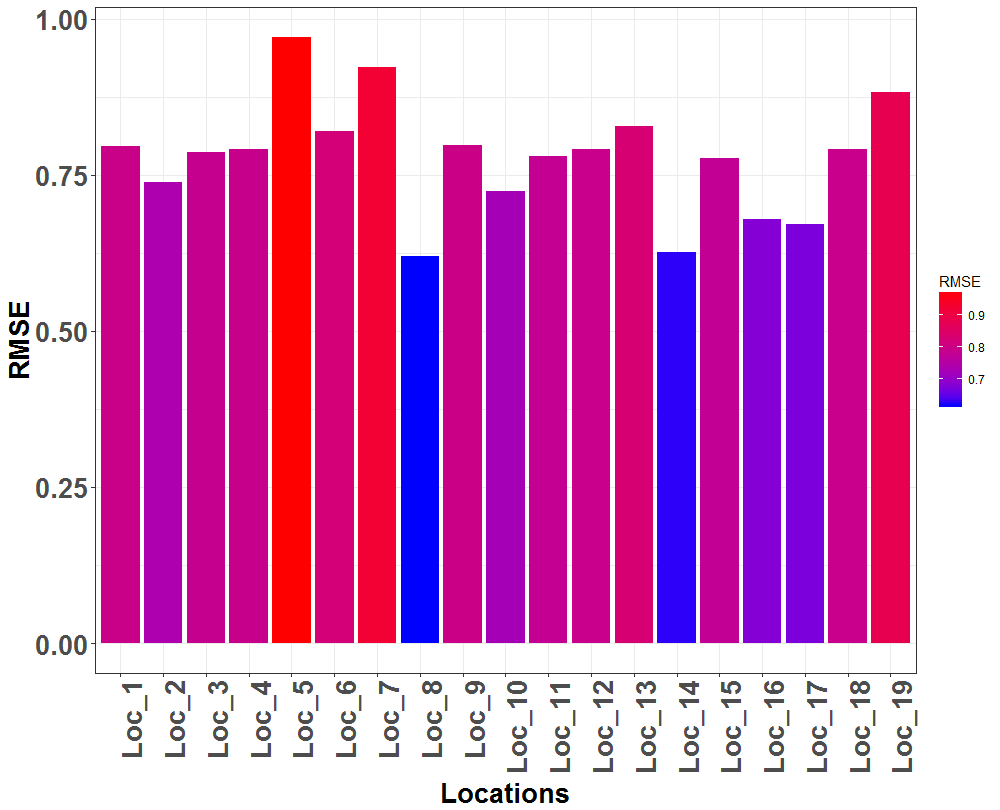
\includegraphics[width=8cm]{RMSE_bar_plots_outage.png} &
 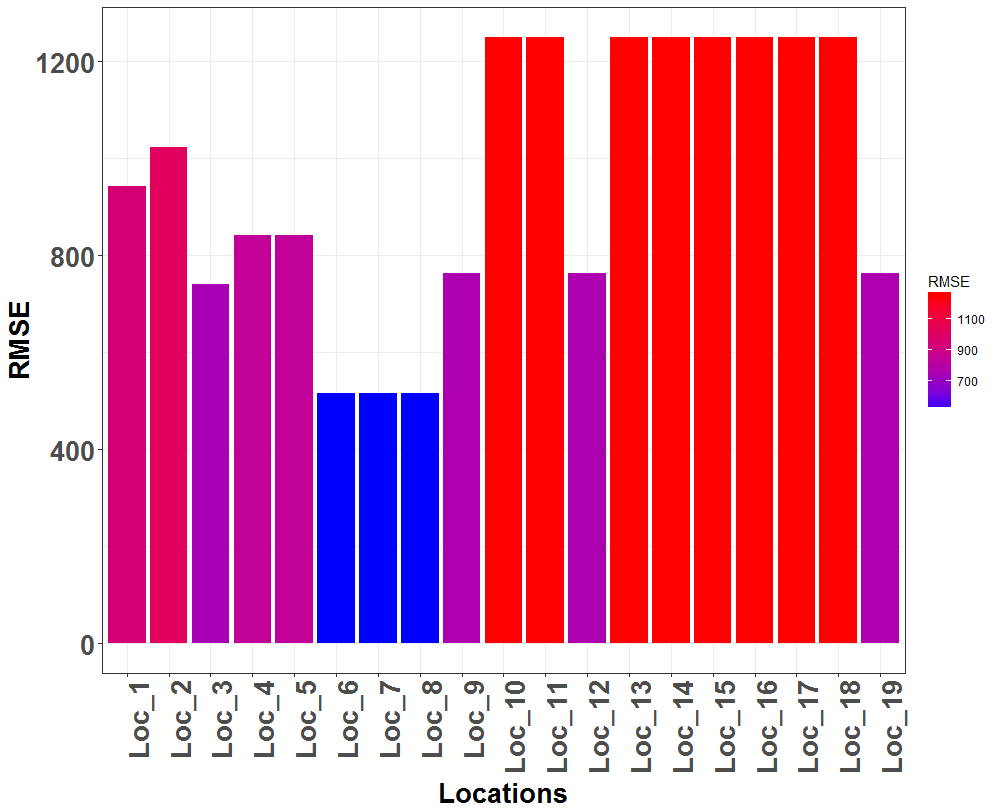
\includegraphics[width=8cm]{RMSE_bar_plots_combined_demand.png}\\
{\Large \bf(a)} & {\Large \bf(b)}\\
\end{tabular}
\caption{RMSE values between actual and forecast values of (a) Task volumes, and (b) Resource demands across different service delivery locations.}
\label{fig4a}
\end{figure*}
This experiment empirically demonstrates that (Figure~\ref{fig4a}) time-series based prediction incur high variability in predicting resource demands, compared to the number of service requests predicted. The root of the variation is multi-factor contribution on the task sequences and resource demand, which are not time continuous. This exercise empirically shows that it is possible to estimate the number of incoming requests with reasonable accuracy using time-series analysis, but to translate the number of service requests to resource demand needs different modeling strategy.   

\subsection{Operating characteristic identification}
We evaluate the effectiveness of distinct operating characteristics detection algorithm, by conducting experiments on synthetic data. The algorithm must identify only those operating modes which exhibit significant differences in their distribution, also uniquely identified by distinct factors. To test the same, we have designed a parametric strategy for synthesizing experimental data. We assume that the data follows normal distribution. There exists $k$ clusters in the experimental data, and for each cluster there exist distinct statistics ($\mu_j, \sigma_j$), where $j={1,\dots,k}$. $\mu_j$ and $\sigma_j$ are the mean and standard deviation of $j^{th}$ cluster respectively. Let $F_i$ is a categorical decision factor, taking $p$ different values. Association of value of $F_i$ with a cluster is described using Multinomial distribution. We assume $k$ = 2, and $p$ = 2.
\par
The parameters for experiment design are $\alpha$, and $Z_D$. Here, $\alpha$ models the confusion between the clusters; i.e., how distinctly the factor is characterizing the operating modes, and $Z_D$ controls the cluster separation. Similarly, parameter ${\alpha}$ determines the confusion matrix between cluster and factor, as described  below:
\begin{center}
\begin{tabular}{c c c}
	           & {\bf cluster - 1}       & {\bf cluster - 2} \\
{\bf factor a} &    $\alpha$         & ($1 - \alpha$) \\
{\bf factor b} &    ($1 - \alpha$)  & $\alpha$ \\
\end{tabular}
\end{center}
$\alpha$ takes values in the range of [0, 1]. $\alpha=1$ signifies one to one correspondence between a cluster and a factor, and $\alpha=0.5$ suggests no correlation between clusters and factors.
\par
The cluster separation is described as $Z_{D} = \dfrac{\vert{\mu}_1 - {\mu}_2\vert}{{\sigma}_1 + {\sigma}_2}$. That is higher value of $Z_D$ higher the separation between clusters.
\begin{figure*}
    \centering
	\begin{tabular}{cc}
	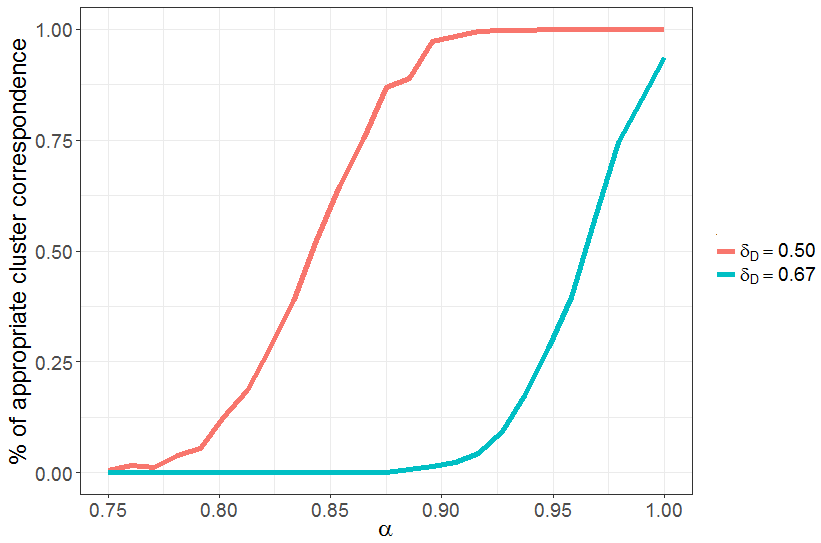
\includegraphics[width=8cm]{fig4a} &
	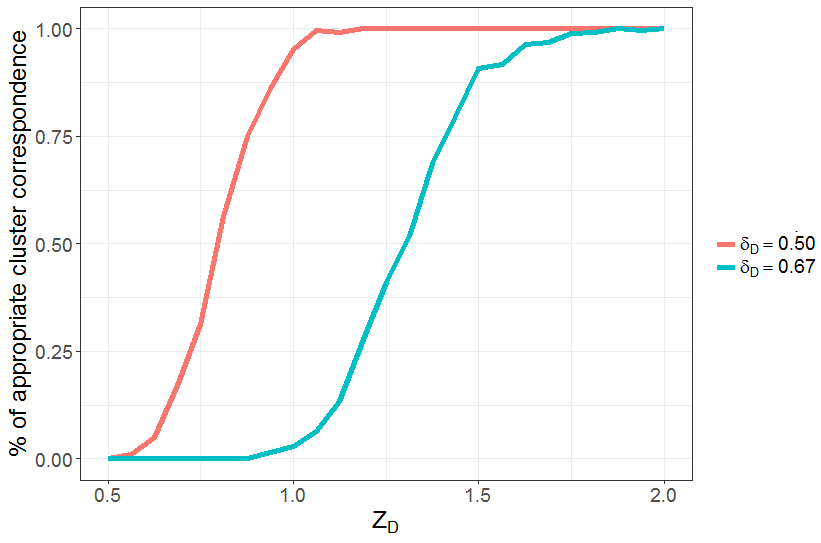
\includegraphics[width=8cm]{fig4b} \\
	{\bf (a)} & {\bf (b)} \\
	\end{tabular}
    \caption{Experimental validation of operating characteristic identification algorithm.}
    \label{fig4}
\end{figure*}

We have carried out experiments with two distinct value of $\delta_D$ to demonstrate its effect on the operating characteristics detection algorithm (section~\ref{subsec:characteristic}). Experimental results (Figure-\ref{fig4}) confirms lower values of $\delta_{D}$ allows identification of finer operating characteristics. Higher values of $\delta_{D}$ identify only well separated operation characteristics, and low confusion on factor values. For robust modeling, high value of $\delta_{D}$ (in the range of $\geq 0.85$) is best suggested.


\subsection{Sequence Generator}
In this section, we study empirically the effect of training data size for reliable estimation of Markov transition matrix. We generate sequences using a finite Markov transition matrix. Finite training data is used to estimate the transition matrix. Frobenius norm of the differences in actual, and estimated Markov transition matrices is used as a measure of convergence of the sequence model. 

\begin{figure}[t]
    \centering
	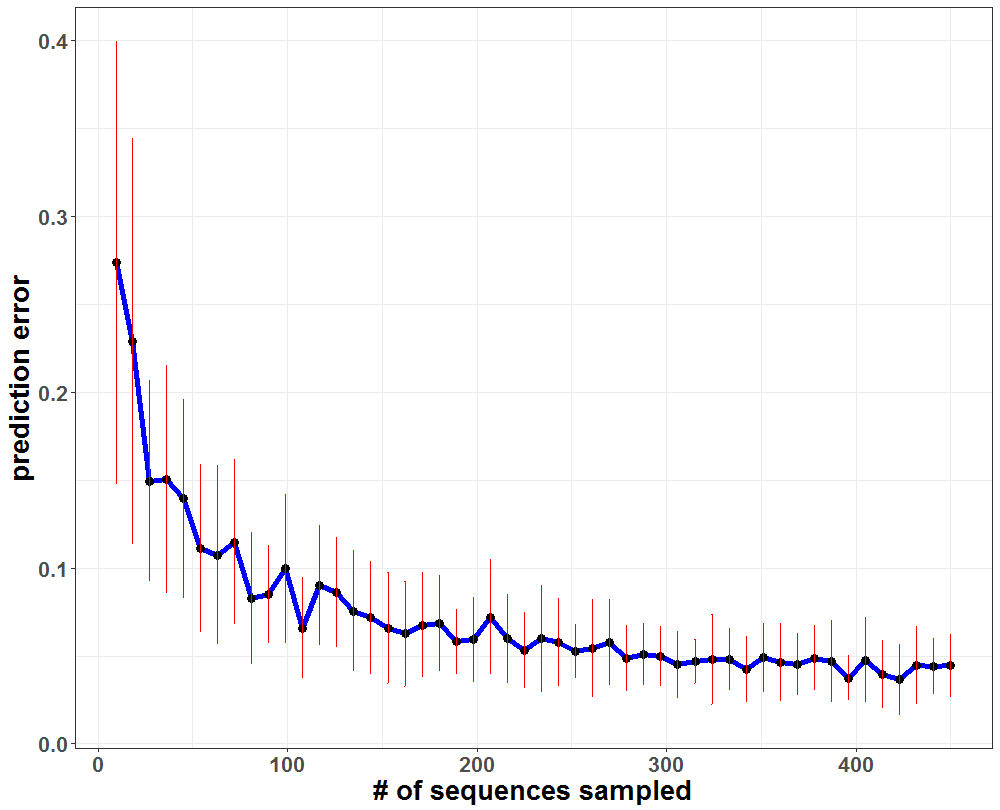
\includegraphics[width=7cm]{markov_sequence}
	\caption{Plot of Markov estimation errors Vs training data size. The experiment involves 50 bootstrap samples, the variations in the estimate are shown as the error bar.}
    \label{fig5}
\end{figure}

Experiment shows the estimation error goes down exponentially with the size of training data. This exponential decay in error estimation guarantees that it is possible to estimate the dynamical system parameters reliably with a moderate size training data set.

\subsection{Prediction Accuracy}
To validate the system performance, we have used data from major event days (i.e., the number of service requests will be high due to some disastrous event like storm, or fire, etc.). 

\begin{figure*}
    \centering
	\begin{tabular}{cc}
		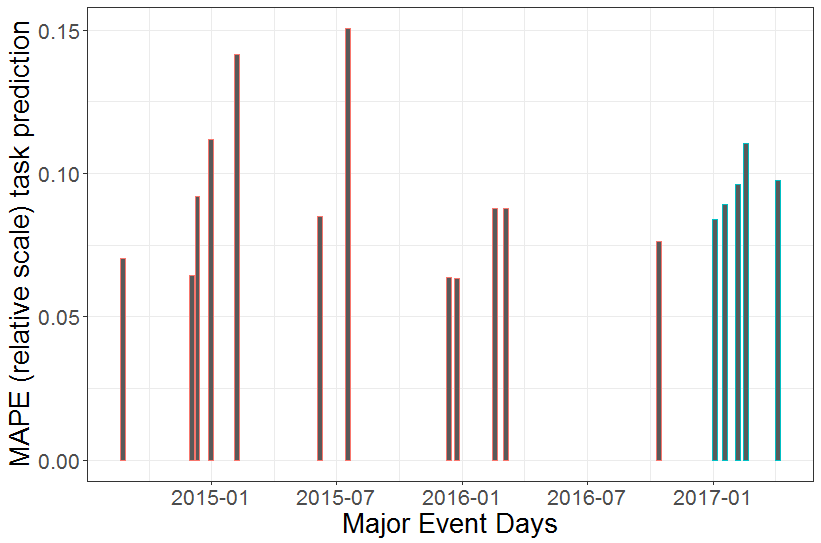
\includegraphics[width=7cm]{fig6a} & 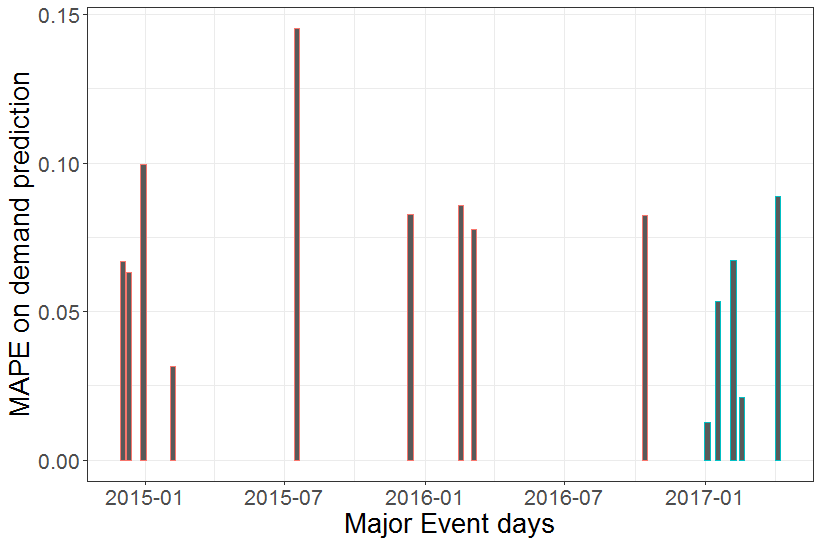
\includegraphics[width=7cm]{fig6b} \\
		{\Large \bf (a)} & {\Large \bf (b)} \\
	\end{tabular}
    \caption{Mean absolute percentage error (MAPE) : (a) for task volume prediction, (b) for resource demand prediction.}
    \label{fig6}
\end{figure*}

Under emergency scenario, the outage volume is significantly high (250 - 1500\% over a regular day's outage count) (Figure~\ref{fig6}). The model is trained on 3 years of historical activity log data. The red bars are high volume outage days with in the 3 years of training data (i.e., in sample data prediction). The green bars are prediction on data, which is excluded from the training (i.e., out sample data prediction). The model shows very consistent performance, showing mean absolute percentage error (MAPE) below 15\%. 
\par 
Unlike the ARIMA analysis in Section~\ref{subsec:timeseries}, the predicted values of resource demand by our model are in consistent with the predicted values of task volume.

\section{Conclusions and Summary}
Here we propose a generic method for demand estimation in a distributed service delivery system. The process template proposed on which different components are integrated are fairly generic, and can be extended to various domains of distributed service delivery. Novel contributions of our methods are, producing sequence of dependent tasks, producing sequence of dependent activities,  generating associated resource demands, and finally producing a measure of uncertainty. This is extremely useful for robust resource planning to allocate resources, for the faster and cost efficient resolution of the service requests. 
\par
The proposed method uses simple Markovian assumption for task sequence and activity sequence generation. This makes the process simple and amenable to mathematical analysis. There are use-cases, where the activity and task sequence exhibits memory, or higher order correlation. The methods can be extended easily to accommodate such sequences generation models. Even with this simple assumption, we have attained a very good prediction accuracy on a real life representative data-set. 
\par
Output from this method can be consumed by an optimization planner for effective planning of resource allocation to service request resolution. The demand prediction using this method, can be carried out at real time, even for inputs with partially observed data. This feature particularly is very useful for making mid-event management decisions under emergency conditions (e.g., in the event of a storm, or earth quake, or fire, etc.).

\bibliographystyle{abbrv}
\bibliography{sigkddExp} 

\end{document}

% End of ltexpprt.tex